\documentclass[10pt]{article}

\usepackage[margin=0.75in]{geometry}
\usepackage{amsmath,amsthm,amssymb}
\usepackage{xcolor}
\usepackage{cancel}
\usepackage{graphicx}
\usepackage{changepage}
\usepackage{circuitikz}
\usepackage{pgfplots}
\usepackage{physics}
\usepackage{hyperref}
\usepackage{siunitx}
\usepackage{fontspec}
\usepackage{relsize}
\usepackage{subfig}
\usepackage{todonotes}
\usepackage{multicol, multirow, booktabs}
\usepackage[breakable]{tcolorbox}
\usepackage[inline]{enumitem}

\theoremstyle{definition}
\newtheorem{problem}{Problem}
\newtheorem{soln}{Solution}
\makeatletter
\newenvironment{subtheorem}[1]{%
  \def\subtheoremcounter{#1}%
  \refstepcounter{#1}%
  \protected@edef\theparentnumber{\csname the#1\endcsname}%
  \setcounter{parentnumber}{\value{#1}}%
  \setcounter{#1}{0}%
  \expandafter\def\csname the#1\endcsname{\theparentnumber.\Alph{#1}}%
  \ignorespaces
}{%
  \setcounter{\subtheoremcounter}{\value{parentnumber}}%
  \ignorespacesafterend
}
\makeatother
\newcounter{parentnumber}

\pgfplotsset{compat=newest}
\usetikzlibrary{lindenmayersystems}
\usetikzlibrary{arrows}
\usetikzlibrary{calc}
\usetikzlibrary{positioning, fit}
\usetikzlibrary{3d, perspective}
\usetikzlibrary{patterns.meta}

\definecolor{incolor}{HTML}{303F9F}
\definecolor{outcolor}{HTML}{D84315}
\definecolor{cellborder}{HTML}{CFCFCF}
\definecolor{cellbackground}{HTML}{F7F7F7}
\newcommand{\ui}{\hat{i}}
\newcommand{\uj}{\hat{j}}
\newcommand{\uk}{\hat{k}}
\newcommand{\ux}{\hat{x}}
\newcommand{\uy}{\hat{y}}
\newcommand{\uz}{\hat{z}}
\newcommand{\primed}[1]{#1^\prime}
\pgfdeclarelayer{background}  
\pgfsetlayers{background,main}
\AtBeginDocument{\RenewCommandCopy\qty\SI}
\newcommand{\justif}[2]{&{#1}&\text{#2}}
\DeclareMathOperator\Arg{Arg}

\makeatletter
\newcommand{\boxspacing}{\kern\kvtcb@left@rule\kern\kvtcb@boxsep}
\makeatother
\newcommand{\prompt}[4]{
    \ttfamily\llap{{\color{#2}[#3]:\hspace{3pt}#4}}\vspace{-\baselineskip}
}

\newcommand{\thevenin}[2]{
  \begin{center}
    \begin{circuitikz} \draw
      (0,0) -- (2,0) to[battery1, l_=$V_{Th}\eq#1$] (2,2) 
      to[resistor, l_=$R_{Th}\eq#2$] (0,2)
      ;
      \draw [o-] (-.07,2.079);
      \draw [o-] (-.07,0.079);
    \end{circuitikz}
  \end{center}
}

\newcommand{\norton}[2]{
  \begin{center}
    \begin{circuitikz} \draw
      (0,0) -- (3,0) to[american current source, l_=$I_{N}\eq#1$] (3,2) -- (0,2) (2,0)
      to[resistor, l=$R_{N}\eq#2$] (2,2)
      ;
      \draw [o-] (-.07,2.079);
      \draw [o-] (-.07,0.079);
    \end{circuitikz}
  \end{center}
}

\newcommand{\highlight}[1]{\colorbox{yellow}{$\displaystyle #1$}}

\newcommand{\ti}[1]{\widetilde{#1}}

\newfontface{\Kaufmann}{Kaufmann}
\DeclareTextFontCommand{\kf}{\Kaufmann}
\newcommand{\scriptr}{\fontsize{12pt}{12pt}\kf{r}}

\newfontface{\KaufmannB}{Kaufmann Bd BT}
\DeclareTextFontCommand{\kfb}{\KaufmannB}
\newcommand{\bscriptr}{\fontsize{12pt}{12pt}\kfb{r}}

\newcommand{\bv}[1]{\mathbf{#1}}

\title{Math 3770H: Assignment II}
\author{Jeremy Favro (0805980) \\ Trent University, Peterborough, ON, Canada}
\date{\today}

\begin{document}
\maketitle

% PROBLEM 1
\begin{problem}
Write the function
$$f(z)=z+\frac{1}{z}\qquad(z\neq 0)$$
in the form $f(z)=u(r,\theta)+iv(r,\theta)$
\end{problem}
\begin{soln}
  Writing $f$ first in polar form to switch to a dependence on $r=\abs{z},\theta=\arctan\left(\Im z/\Re z\right)$,
  $$z=re^{i\theta}=r\cos\theta+ir\sin\theta.$$
  This is actually really nice here as it means we can easily write the inverse without using a fraction,
  $$z^{-1}=r^{-1}e^{-i\theta}=r^{-1}\cos\left(-\theta\right)+ir^{-1}\sin\left(-\theta\right).$$
  Which can be reworked further using the even/odd nature of $\cos$ and $\sin$ respectively giving:
  \begin{align*}
    f(z) & =r\cos\theta+ir\sin\theta + r^{-1}\cos\theta-ir^{-1}\sin\theta      \\
         & =r\cos\theta+r^{-1}\cos\theta + ir\sin\theta -ir^{-1}\sin\theta     \\
         & =\left(r+r^{-1}\right)\cos\theta +  \left(r+r^{-1}\right)\sin\theta
  \end{align*}
\end{soln}
\newpage

% PROBLEM 2
\begin{problem}
Sketch the region onto which the sector $r \leq 1$, $0 \leq \theta \leq \pi/4$ is mapped by the transformation
\begin{center}
  \begin{enumerate*}[label=(\alph*)]
    \item $w = z^2$;\qquad~
    \item $w = z^3$;\qquad~
    \item $w = z^4$.
  \end{enumerate*}
\end{center}
\end{problem}
\begin{soln}
  Generally the transform $w=z^n$ will give $w=r^ne^{in\theta}$, just by exponentiation laws. Our original region looks like:
  \begin{center}
    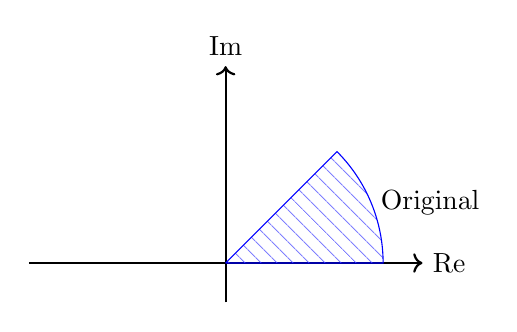
\begin{tikzpicture}[scale=2]
      \draw[->,thick] (-1.25,0)--(1.25,0) node[right]{$\Re$};
      \draw[->,thick] (0,-.25)--(0,1.25) node[above]{$\Im$};
      \filldraw[pattern={Lines[angle=-45,distance=4pt]}, draw=blue, pattern color=blue!50!white] (0,0) -- (1,0) arc (0:45:1) node[midway, right]{Original} -- (0,0);
    \end{tikzpicture}
  \end{center}
  Because our region only extends out to $r=1$ the radius won't change.
  \begin{enumerate}[label=(\alph*)]
    \item ~\begin{center}
            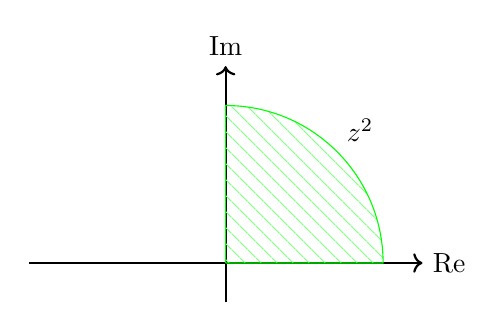
\begin{tikzpicture}[scale=2]
              \draw[->,thick] (-1.25,0)--(1.25,0) node[right]{$\Re$};
              \draw[->,thick] (0,-.25)--(0,1.25) node[above]{$\Im$};
              \filldraw[pattern={Lines[angle=-45,distance=4pt]}, draw=green, pattern color=green!50!white] (0,0) -- (1,0) arc (0:{2*45}:1) node[midway, above right]{$z^2$} -- (0,0);
            \end{tikzpicture}
          \end{center}
    \item ~\begin{center}
            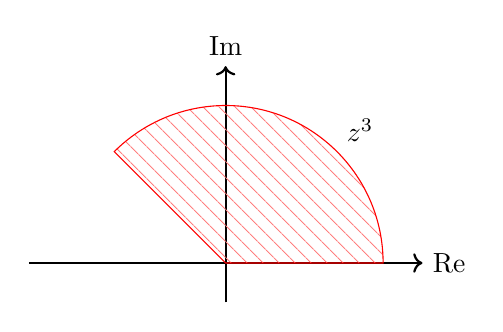
\begin{tikzpicture}[scale=2]
              \draw[->,thick] (-1.25,0)--(1.25,0) node[right]{$\Re$};
              \draw[->,thick] (0,-.25)--(0,1.25) node[above]{$\Im$};
              \filldraw[pattern={Lines[angle=-45,distance=4pt]}, draw=red, pattern color=red!50!white] (0,0) -- (1,0) arc (0:{3*45}:1) node[pos=0.333, above right]{$z^3$} -- (0,0);
            \end{tikzpicture}
          \end{center}
    \item ~\begin{center}
            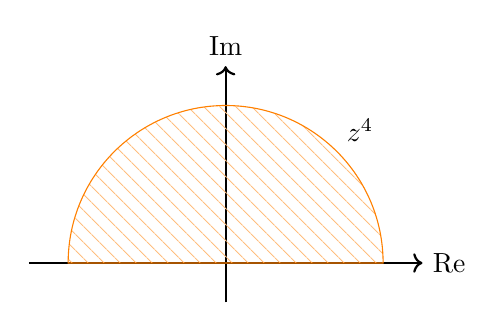
\begin{tikzpicture}[scale=2]
              \draw[->,thick] (-1.25,0)--(1.25,0) node[right]{$\Re$};
              \draw[->,thick] (0,-.25)--(0,1.25) node[above]{$\Im$};
              \filldraw[pattern={Lines[angle=-45,distance=4pt]}, draw=orange, pattern color=orange!50!white] (0,0) -- (1,0) arc (0:{4*45}:1) node[pos=0.25, above right]{$z^4$} -- (0,0);
            \end{tikzpicture}
          \end{center}
  \end{enumerate}
\end{soln}
\newpage

% PROBLEM 3
\begin{problem}
Use definition (2), Sec.15, of the limit to prove that
\begin{center}
  \begin{enumerate*}[label=(\alph*)]
    \item $\lim_{z\to z_0}\Re z = \Re z_0$;\qquad~
    \item $\lim_{z\to z_0}\overline{z}=\overline{z_0}$;\qquad~
    \item $\lim_{z\to 0}\frac{\overline{z}^2}{z}=0$.
  \end{enumerate*}
\end{center}
\end{problem}
\begin{soln}~
  \begin{enumerate}[label=(\alph*)]
    \item Let $\epsilon>0$. Suppose $\abs{z-z_0}<\delta$. If we take $z=x+iy$ and $z_0=x_0+iy_0$ then we have
          $$\abs{\Re z-\Re z_0}=\abs{x-x_0}\leq \abs{z-z_0}.$$
          We can make that last statement because
          $$\abs{x-x_0}\leq \abs{x-x_0+iy-iy_0}=\abs{z-z_0}.$$
          This means that
          $$\abs{\Re z-\Re z_0}=\abs{z-z_0}\leq \delta$$
          by the $\epsilon-\delta$ definition we are using. Having this means that provided
          $\abs{z-z_0}\leq \delta=\epsilon$, then $\abs{\Re z-\Re z_0}<\epsilon$ by transitivity.
    \item Let $\epsilon>0$. Suppose $\abs{z-z_0}<\delta$. We have
          $$\abs{\overline{z}-\overline{z_0}}=\abs{\overline{z-z_0}}=\abs{z-z_0}<\delta$$
          all by properties of the complex conjugate. So provided $\abs{z-z_0}<\delta=\epsilon$, then
          $\abs{\overline{z}-\overline{z_0}}<\epsilon$.
    \item Let $\epsilon>0$. Suppose $\abs{z-z_0}<\delta$. We have
          $$\abs{\frac{\overline{z}^2}{z}-\frac{\overline{z_0}^2}{z_0}}=\abs{\frac{\overline{zz}}{z}-\frac{\overline{z_0z_0}}{z_0}}$$
    
    
    $\lim_{z\to 0}=0$.
  \end{enumerate}
\end{soln}

% PROBLEM 4
\begin{problem}
With the aid of the theorem in Sec. 17, show that when
$$T(z)=\frac{az+b}{cz+d}\qquad (ad-bc)\neq0$$
\begin{enumerate}[label=(\alph*)]
  \item $\lim_{z\to\infty}T(z)=\infty\quad \text{if } c=0$;
  \item $\lim_{z\to\infty}T(z)=\frac{a}{c}\quad\text{and}\quad\lim_{z\to-d/c}T(z)=\infty\quad\text{if } c\neq 0$
\end{enumerate}
\end{problem}
\begin{soln}
\end{soln}

% PROBLEM 5
\begin{problem}
Use the method in Example 2, Sec. 19, to show that $f(z)$ does not exist at any point
$z$ when
\begin{enumerate*}[label=(\alph*)]
  \item $f(z)=\Re z$;\qquad~
  \item $f(z)=\Im z$.
\end{enumerate*}
\end{problem}
\begin{soln}
\end{soln}

% PROBLEM 6
\begin{problem}
Use the theorem in Sec. 24 to show that each of these functions is differentiable in the
indicated domain of definition, and also to find $\primed{f}(z)$:
\begin{enumerate}[label=(\alph*)]
  \item $f(z)=1/z^4$ $(z\neq 0)$;
  \item $f(z)=e^{-\theta}\cos\left(\ln r\right)+ie^{-\theta}\sin\left(\ln r\right)$ $(r>0. 0<\theta<2\pi)$.
\end{enumerate}
\end{problem}
\begin{soln}
\end{soln}

% PROBLEM 7
\begin{problem}
With the aid of the theorem in Sec. 21, show that each of these functions is nowhere
analytic:
\begin{enumerate*}[label=(\alph*)]
  \item $f(z)=xy+iy$;\qquad~
  \item $f(z)=2xy+i(x^2-y^2)$;\qquad~
  \item $f(z)=e^ye^{ix}$.
\end{enumerate*}
\end{problem}
\begin{soln}
\end{soln}

% PROBLEM 8
\begin{subtheorem}{problem}
  \begin{problem}
  Let the function $f (z) = u(x, y) + iv(x, y)$ be analytic in a domain $D$, and consider the
  families of level curves $u(x, y) = c_1$ and $v(x, y) = c_2$ , where $c_1$ and $c_2$ are arbitrary
  real constants. Prove that these families are orthogonal. More precisely, show that if
  $z_0 = (x_0,y_0)$ is a point in $D$ which is common to two particular curves $u(x, y) = c_1$
  and $v(x, y) = c_2$ and if $\primed{f}(z_0)\neq0$, then the lines tangent to those curves at $(x_0,y_0)$ are
  perpendicular.
  \end{problem}
  \begin{problem}
  Sketch the families of level curves of the component functions $u$ and $v$ when
  $f(z) = 1/z$, and note the orthogonality described in Exercise 2.
  \end{problem}
\end{subtheorem}
\begin{subtheorem}{soln}
  \begin{soln}
  \end{soln}
  \begin{soln}
  \end{soln}
\end{subtheorem}
\end{document}